\subsection{Overview}
Given the nature of the application, a three layer approach has been chosen.\newline
\begin{figure}[h!]
	\centering
	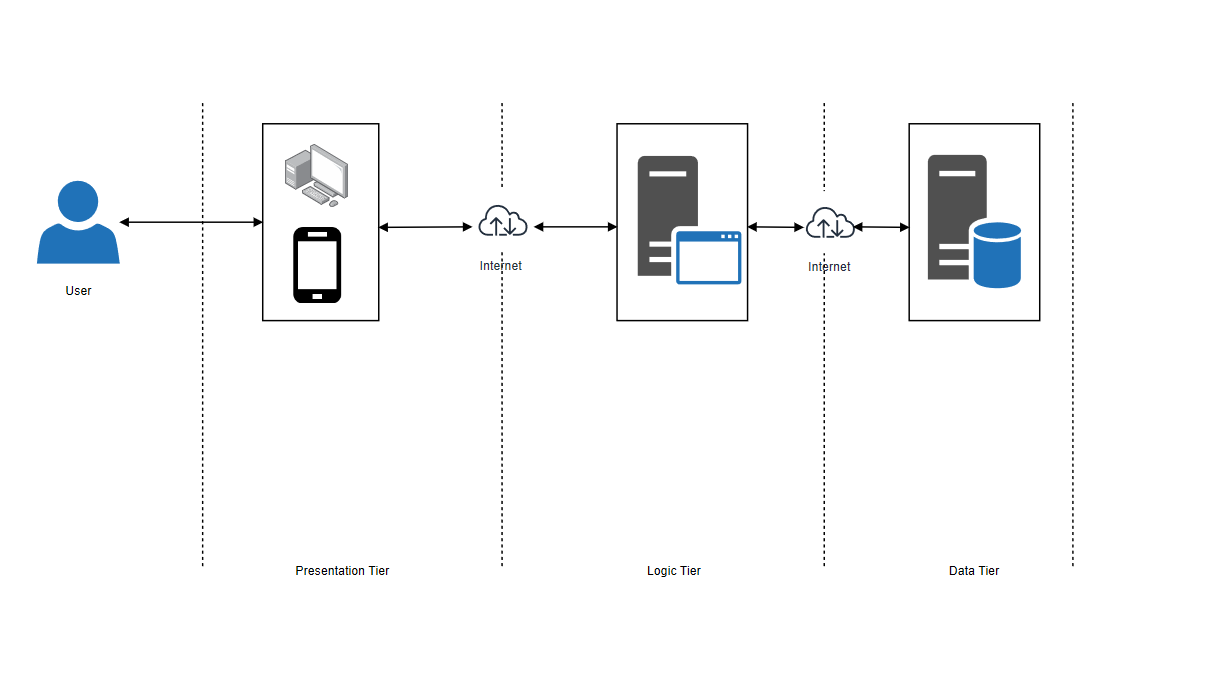
\includegraphics[width=\textwidth]{Images/three_layer}
	\caption{Three layer structure}
\end{figure}
\newline
As shown by the image above, the three layers consist in the presentation tier, the logic tier and the data tier
\begin{itemize}
\item Presentation Tier: consists of the user interfaces for all of the three clients (RegularUser, Policeman and MunicipalAuthority) and is used by the user to interact with both the application logic and Google Mapd APIs \newline
\item Logic Tier: consists of the servers used to control the functionalities of the application, interacts with both the presentation and data tiers \newline
\item Data Tier: consists of the database server (where both user data and data generated by the application are stored), interacts only with the logic tier \newline
\end{itemize}
\newpage
\subsection{Component view}

The following diagram represents the interface structure of the system, focusing on both the application server structure. \newline
\begin{figure}[h!]
	\centering
	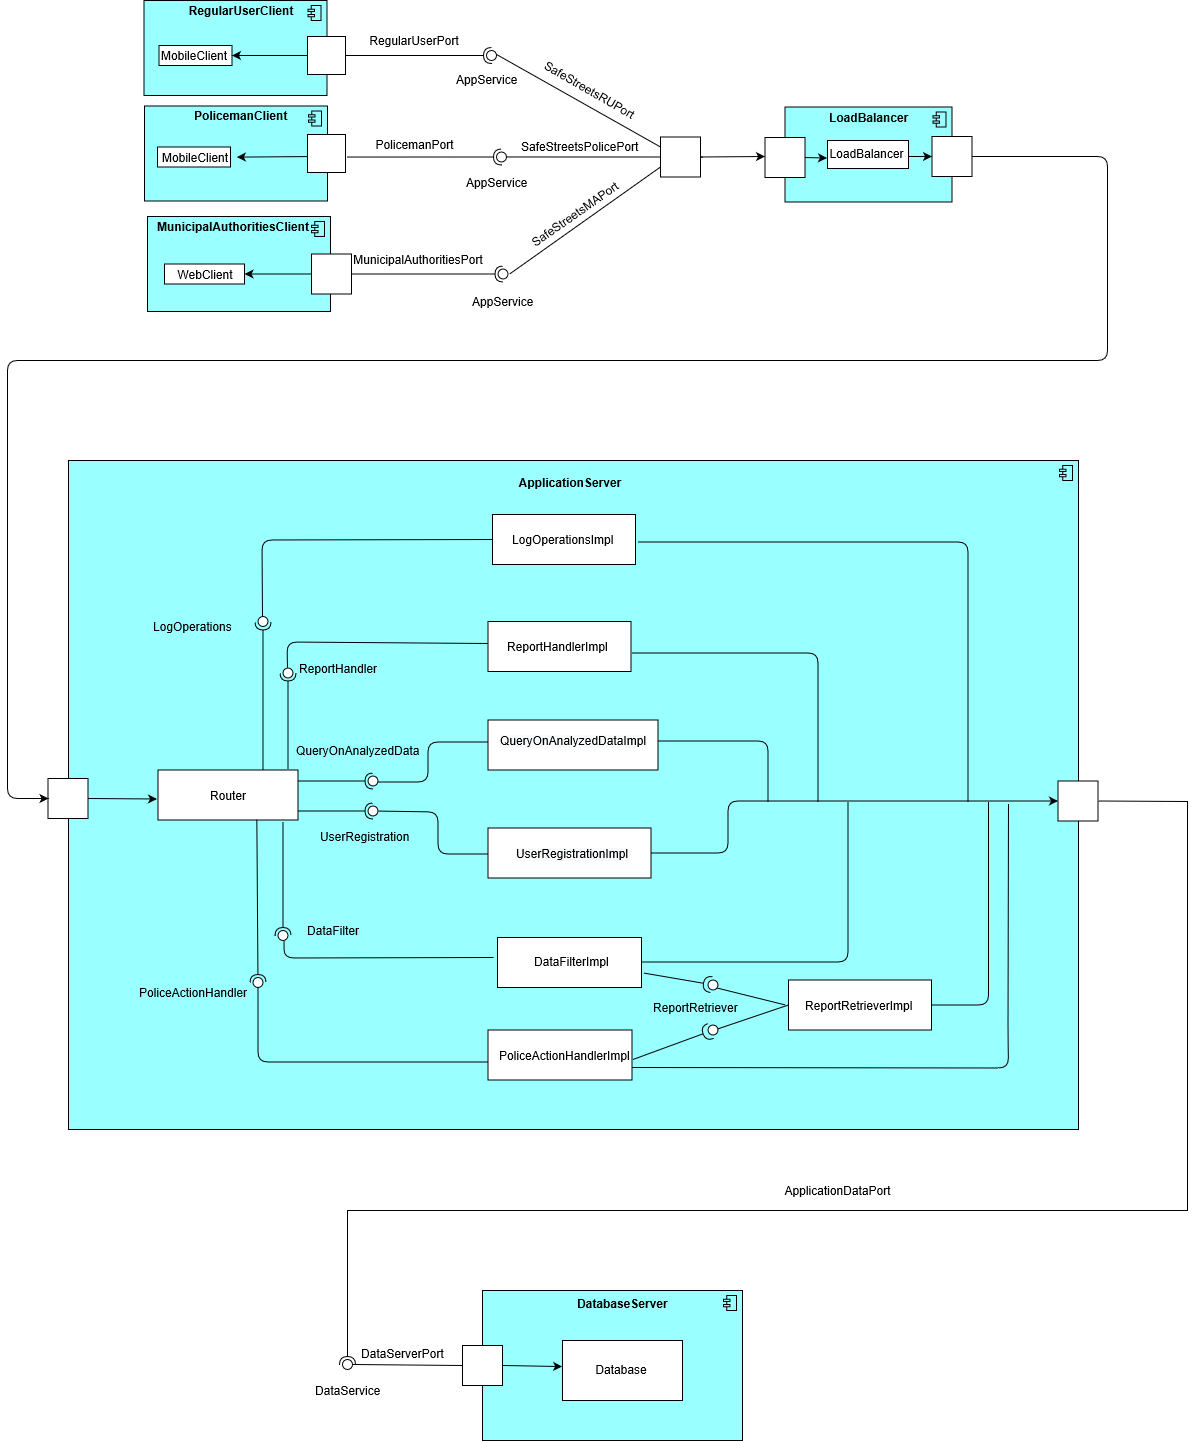
\includegraphics[width=\textwidth]{Images/component_diagram_beta}
	\caption{Component diagram}
\end{figure}

As shown above, the application logic is stored on the application server, while the clients just contain what is mandatory in order to contact the application server (thin client).\\
We will now proceed to give a brief summary of the role of the components listed above:
\begin{itemize}
\item QueryOnAnalizedData: allows the RegularUser profiles to access data about the reports in a certain area or other information already analized by the MunicipalAuthorities
\item PoliceAction: allows the policemen to take action on user made reports or to compile reports themself. The actions performed by the police consist in compiling reports (of which they will take care right away), marking themselves as dispatched towards a report, mark a report as wrong or signal that a traffic ticket has been written as a consequence of a reported traffic violation
\item RetrieveEquiReports: this component is mainly used by PoliceAction in order to retrive all reports that are about the same violation (not just violation type, but also time, plate and location) as a given one. 
\item SendReports: this component allows users to submit the reports about traffic violations that they write. The reports are authenticated and then strored inside the application DB
\item UserRegistration: this component allows the registration of all types iof users. Note that, while RegularUser profiles registration is done by the user themselves, Authority profiles (Policeman and MunicipalAuthority) can only be registered by a system admin
\item LogOperations: this component takes care of the login and logut operations for all types of User profiles
\item QueryOnData: allows MunicipalAuthority profiles to perform data-mining activities,  as well as add information from the municipality DB of crashes and cross-analyze them with user-submitted reports
\end{itemize}
The logic of the application works based on the afromentioned components: they grant all the functionality needed to satisfy the system's goals (for a more in-depth analysis see chapter 4).
In the next two pictures more information about the system will be provided via a more accurate version of the class diagram presented in the RASD and a schema about the relationship between the classes interfaces and implementations of said interfaces. Please note that the "Device" class and the classes that extend it are not reported in the diagram since they are not relevant to the purposes of this description. For any further information about these classes refer to the Class diagram in the RASD.

\begin{figure}[h!]
	\centering
	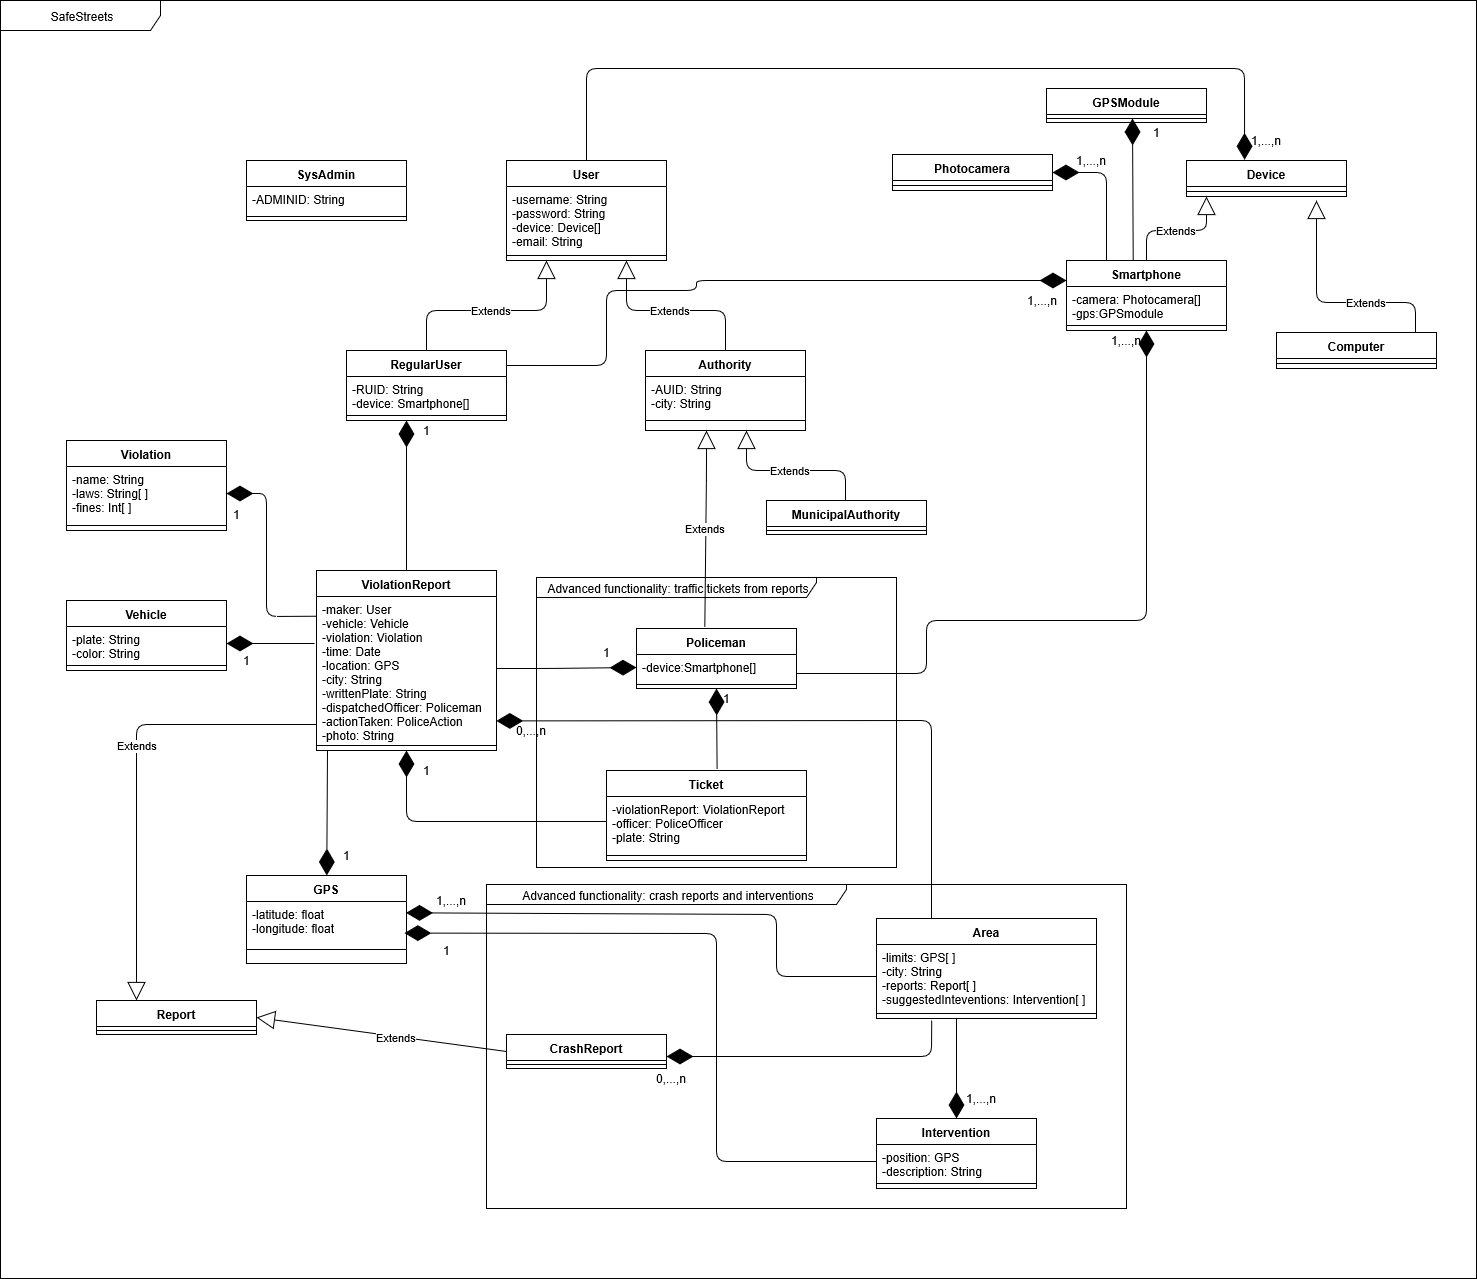
\includegraphics[angle=90, scale=0.40]{Images/ADV_class_diagram}
	\caption{Class diagram}
\end{figure}
\newpage

\begin{figure}[h!]
	\centering
	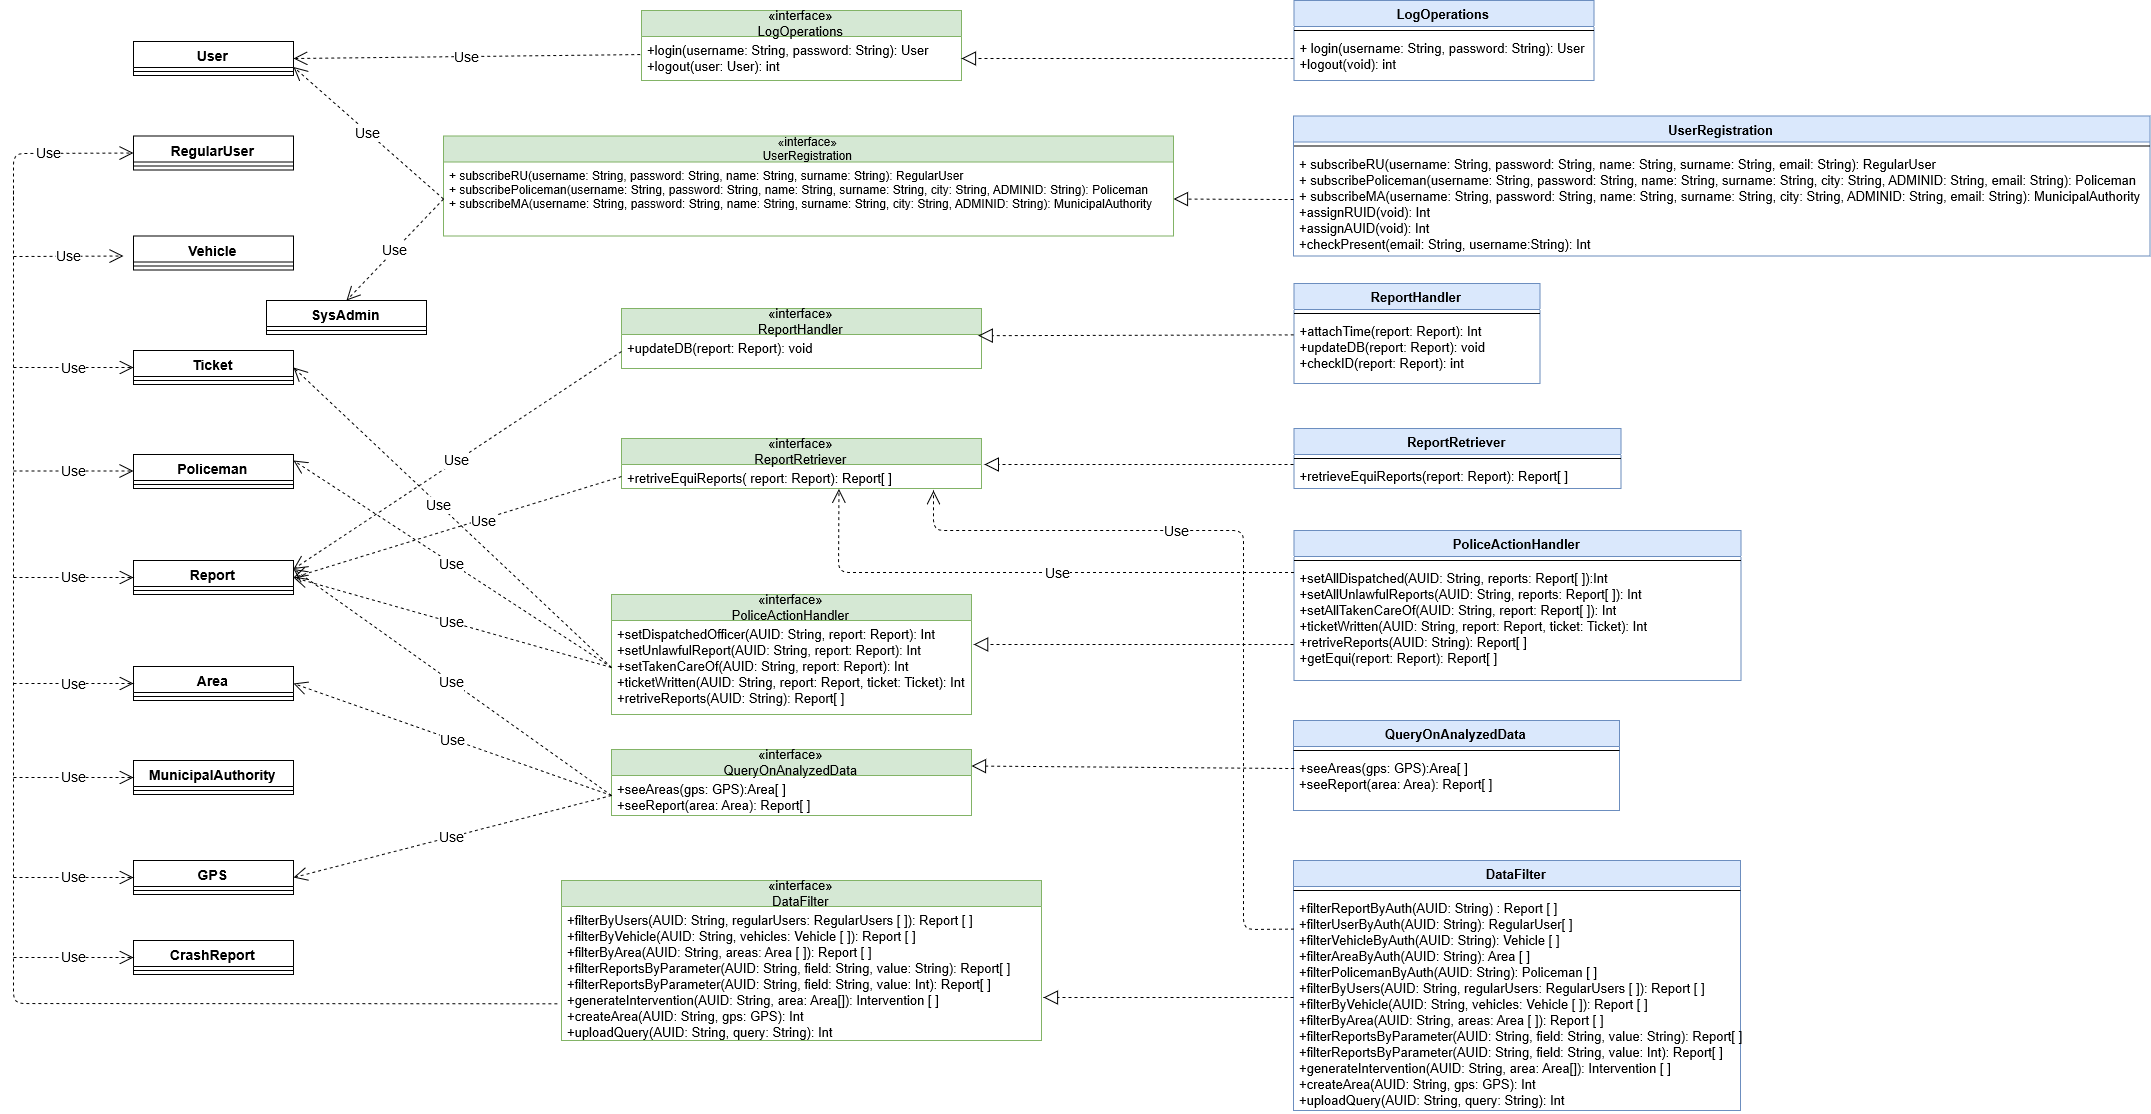
\includegraphics[angle=90, scale=0.28]{Images/component_class_relation}
	\caption{Relation between components and already specified classes}
\end{figure}
\newpage
\subsection{Deployment view}

\begin{figure}[h!]
	\centering
	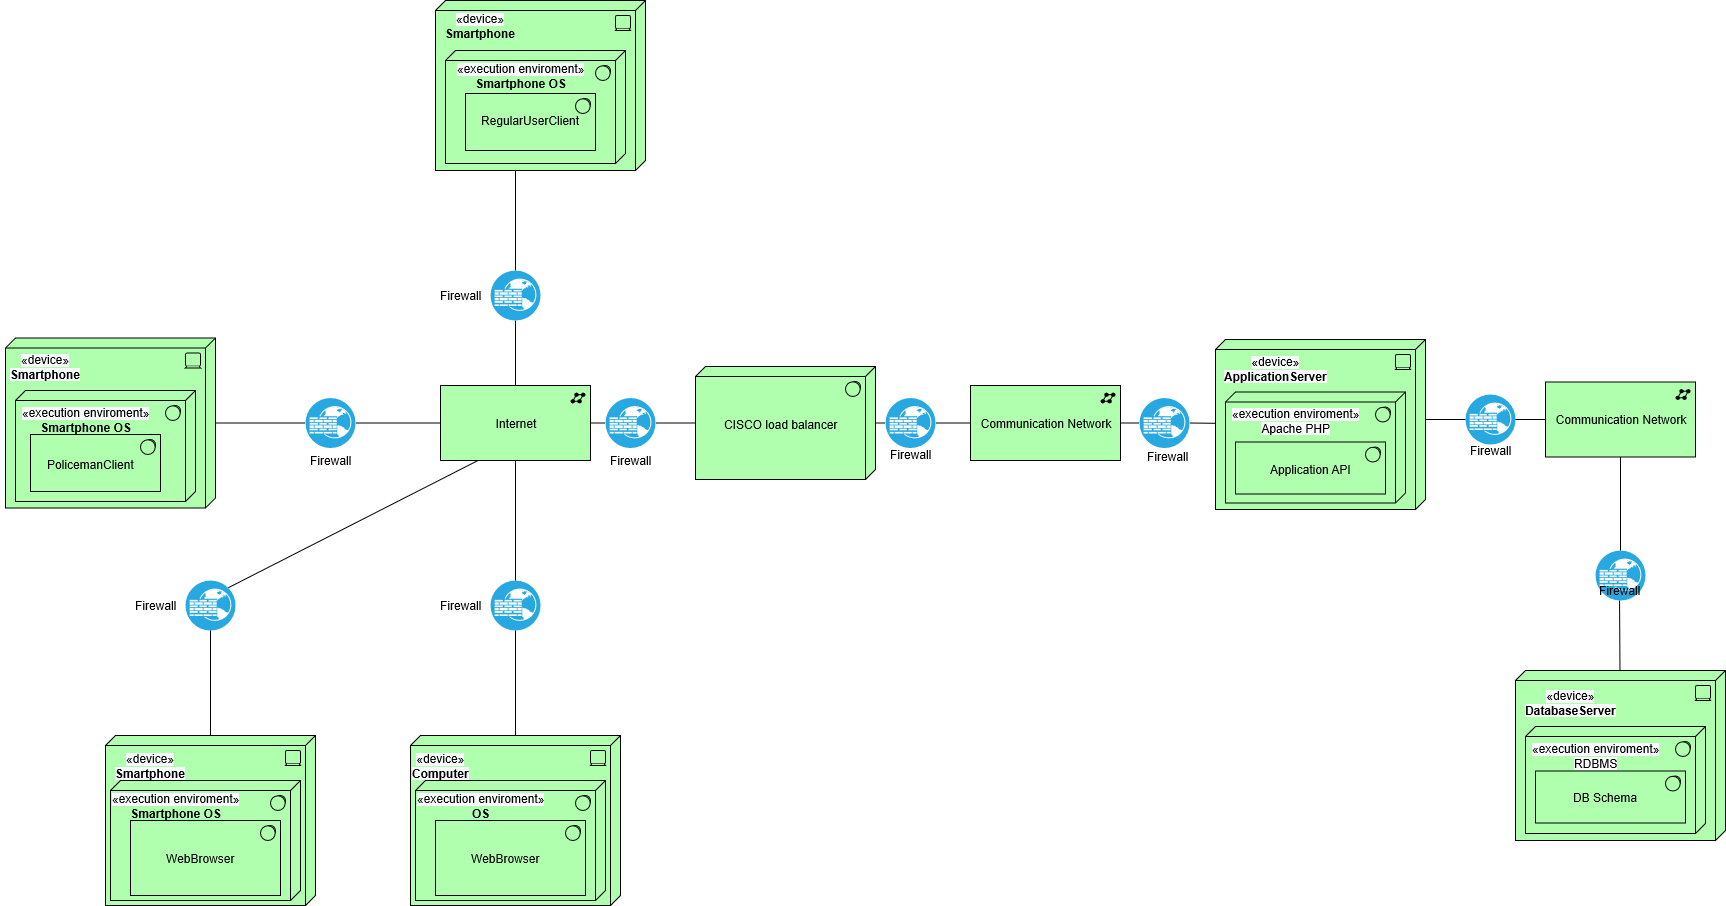
\includegraphics[width=\textwidth]{Images/physical_view}
	\caption{Physical view}
\end{figure}

The image above shows the system's architecture from a physical standpoint.
Components:
\begin{itemize}
\item Smartphone: Device used by both RegularUser and Policeman users type to interact with the application. Two different clients will be developed: one for regular users, that will allow them to look at already analyzed data and submit reports, and a different one for policemen, that will allow the officers make reports (upon which they will take actions right away) and take actions on reports
\item Computer: device used by MunicipalAuthorities users. They will interact with the application via a web page, that will allow them to interact in various ways with the Reports submitted by the other users.
\item Application server: this server contains the application logic and will interact with the different clients in a client-server way.
\item DatabaseServer: this server contains the actual data, both about the registered users and related to the user submitted reports, the actions taken by the police and the results of the data mining operations done by municipal authorities
\end{itemize}
Please note that Google servers have not been included, since those servers will not be involved in the system deployment
\newpage
\subsection{Runtime view}
\newpage
\subsection{Interfaces}
\begin{figure}[h!]
	\centering
	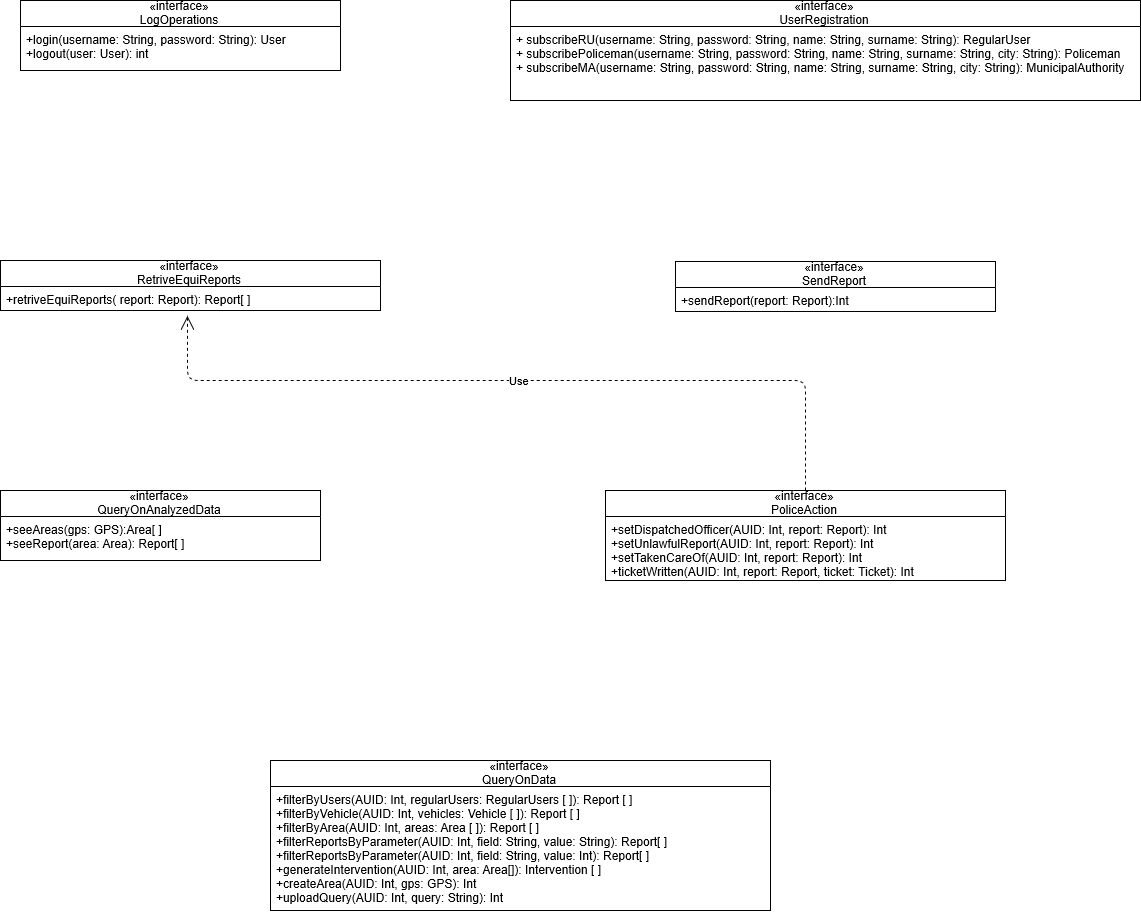
\includegraphics[width=\textwidth]{Images/interface_diagram}
	\caption{Components' interfaces}
\end{figure}
Other than the relation between PoliceAction and RetriveEquiReports, already explained in section 2.2, it is worth noting that the interfaces don't actually expose all the methods of the objects that implement them. This choiche was made in order to hide the methods that will be colled only from inside the object in which they are defined.
\newpage 
\subsection{Architectural and implementative styles and patterns}
\subsubsection{Architectural style}
\begin{itemize}
	\item Client-server:given the nature of the application, a distibuted system in which data submitted by some users has to be accessible by other users, the figure of a mediator becomes necessary. Therefore a client-server architecture seems is a good solution
	\item Thin client: in the afromentioned client-server architecturethe role of the server is more than just a message manager. As a matter of fact, the server also takes care of the application logic, allowing a light client
	\item Three tiers architecture: given the client server with thin client architecture described, the most natural solution is a three tier architecture in which the presentation layer is on the client, the application layer on the application server and the data layer on the database server 
\end{itemize}

